\section{September 2026 Public Release}
\label{sec:public-release}

The September 30 release provides one generic configuration and a native
sheet-assembly command. Parameter-search scripts, experiment and replay
commands, external automation drivers, and the bottom-up hierarchical
welding and repair runners have been removed. The versioned C API,
including its existing option structures, is preserved. Direct grid meshing,
registration, unrolling, and the optional quad-ribbon path remain available.
The research results elsewhere in this report describe the August campaigns;
the run in this section is the measured result of the public configuration.

\subsection{One Configuration and a Staged Assembler}

\path{configs/default.json} supplies the shared configuration, with
\path{configs/axis.csv} carrying the reference axis. The initial calibration
uses PHerc0139: axis $(y,x)=(3405,2878)$, wrap spacing 9.5 coarse voxels,
eight worker threads, and a 900-second repair budget. The input pile
determines the region; the configuration does not impose a hidden crop.
Users must set local CT and executable paths and replace the geometry
calibration when changing datasets.

The command \texttt{sheet\_assemble} accepts a mesh-pile directory, an output
directory, and an optional configuration path. It cleans and flattens charts,
measures cross-cube relations, resolves their poses, places them in a shared
winding-aware domain, admits additional charts, and repairs UV seam, contact,
and metric defects. An audit then accounts for the recorded source inventory
and checks the resulting embedding before export and CT baking. Saved
placement checkpoints support resumption; named stage stops and review
commands support inspection. Repair changes the developed coordinates while
preserving the represented source geometry in three dimensions.

\subsection{PHerc0139 \texorpdfstring{$4\times5\times5$}{4x5x5} Reference Check}

The check uses the saved \texttt{head\_39e72d0\_20260826} mesh pile: 100
cubes of $128^3$ voxels spanning the half-open bounds
$z=[4352,4864)$, $y=[3072,3712)$, and $x=[2560,3200)$.
Assembly completes through audit. All 916,995 source faces are accounted
for, and the represented source vertices are unchanged. Table~\ref{tab:release-audit}
reports the remaining limitations.

\begin{table}[t]
  \caption{Public-configuration reference check, September 30, 2026.
  Area coverage is measured against the recorded source inventory,
  not the raster's bounding rectangle.}
  \label{tab:release-audit}
  \centering
  \small
  \begin{tabular}{@{}lr@{}}
    \toprule
    Measure & Result \\
    \midrule
    Source faces accounted for & 916,995 / 916,995 \\
    Represented source faces & 646,199 \\
    Represented source area & 47.385\% \\
    Placed / unplaced / excluded charts & 356 / 406 / 21 \\
    Invalid faces / strict metric failures & 0 / 0 \\
    Overlapping triangle pairs & 171 \\
    Represented continuity components & 233 \\
    Geometry qualified & No \\
    \bottomrule
  \end{tabular}
\end{table}

The configuration is a usable starting point, but this result is
\emph{not geometry-qualified}: its coverage is below the audit's 85\%
minimum and contacts remain. A successful command exit records processing
completion, not geometric acceptance. This check does not reproduce the
earlier checkpoint-58 atlas or the August quad-ribbon campaigns, which use
different inputs and workflows.

\begin{figure*}[t]
  \centering
  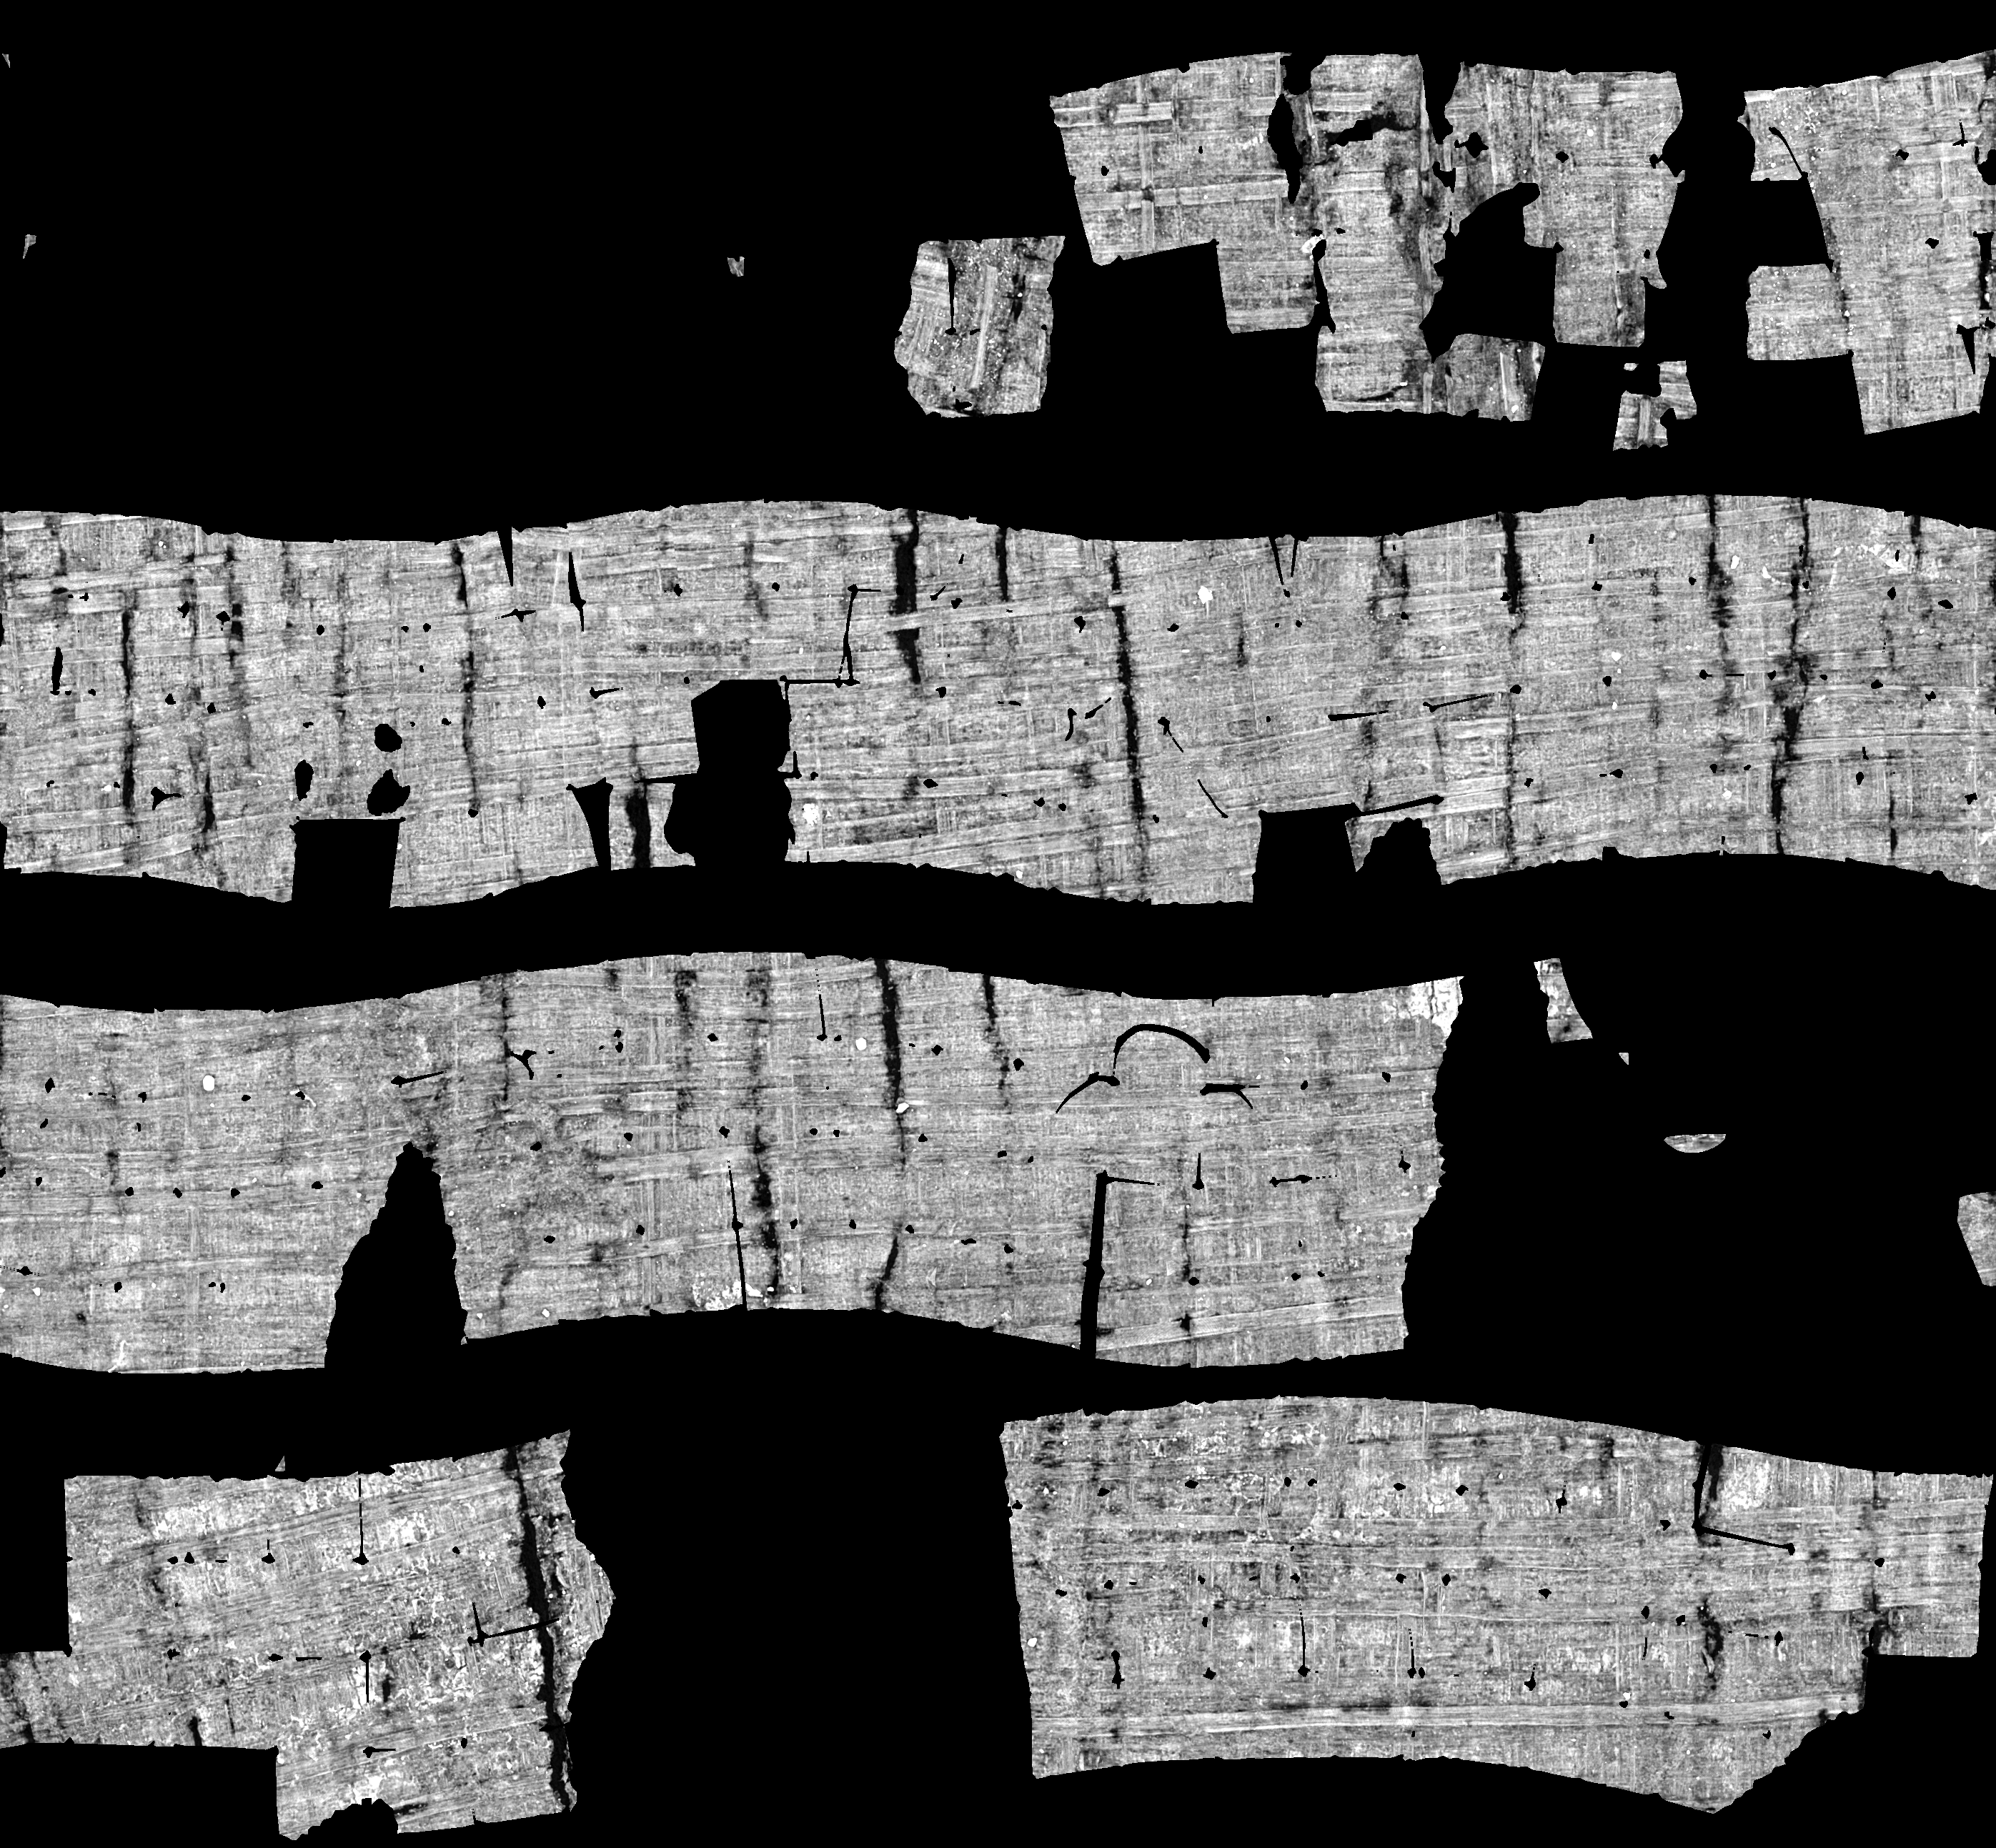
\includegraphics[width=0.94\textwidth]{figures/public_release_4x5x5.png}
  \caption{\textbf{The public-configuration PHerc0139 $4\times5\times5$
  sheet.} CT sampled through the saved repaired VMESH, with the native
  $11{,}170\times642$ raster wrapped into four consecutive rows for viewing.
  The row breaks are display breaks, not inferred seams. The sheet is partial
  (47.385\% source-area coverage), and 171 overlapping triangle pairs remain.
  Black includes unrepresented material and boundary faces whose sampling
  range reaches beyond the available CT cubes. This is the September
  reference check, distinct from the August exhibits.}
  \Description{Four consecutive grayscale strips of CT-textured papyrus on
  a black background. Long central fragments show surface fibres and cube
  seams; separated fragments and black gaps remain at the ends and within
  the partial sheet.}
  \label{fig:public-release-sheet}
\end{figure*}

\paragraph{Texture and evidence.}
Figure~\ref{fig:public-release-sheet} is baked directly from the saved
repaired VMESH without repacking its pieces. Sampling uses one pixel per
coarse voxel, nine samples over $\pm4$ voxels along the surface normal,
and a fixed 8-bit display window of $[47,193]$. This window is an explicit
preview setting; it does not change the assembly audit.
All 100 matching RAW cubes contain CT data. The baker leaves 18,456 boundary
faces unpainted because their sampling range reaches absent neighbouring
cubes; every painted face has the required RAW support. The native coverage
mask separately labels 38,630 pixels of bounded raster crack or pinhole fill.
The committed release evidence index retains the complete audit, bake
coverage report, raster grid, input and artifact hashes, and commands.

\paragraph{Validation.}
The Windows Release CMake build, optional native quad-ribbon build, install
check, and all 16 CTest checks pass. This validates the build and interface
contracts; it does not convert the partial sheet into a qualified unwrapping.
